\section{Introduction}

\begin{frame}{ML-based NIDS Workflow: Train $\rightarrow$ Validate $\rightarrow$ Test $\rightarrow$ Deploy}
    \small
    \begin{columns}[T,onlytextwidth]

        \column{0.55\linewidth}
        \begin{itemize}
            \setlength\itemsep{0.9em}

            \item<1-> The model is trained on a training set
                  \textbf{\(\mathcal{D}_{\text{train}}\)}.

            \item<2-> A separate validation split
                  \textbf{\(\mathcal{D}_{\text{val}}\)} to refine the model
                  hyperparameters.

            \item<3-> A final test set, \textbf{\(\mathcal{D}_{\text{test}}\)},
                  measures performance on unseen data.

            \item<4-> The selected model is deployed to monitor live traffic.
        \end{itemize}

        \only<2>{%
            \vspace{-7em}
            \setbeamercolor{focusbox}{use={structure,normal text},
                fg=structure.fg,
                bg=structure.fg!12!normal text.bg}
            \begin{beamercolorbox}[wd=\linewidth,sep=1ex,rounded=true]{focusbox}
                \small
                \textbf{Hyperparameters:} settings chosen before training that
                influence model behavior.\\
                \textbf{Example}: In RF, too few trees can give unstable
                predictions, while too many can increase computation and overfit
                the training data.
            \end{beamercolorbox}
        }

        \column{0.42\linewidth}
        \begin{figure}
            \centering
            \includegraphics<1>[width=\linewidth]{figures/introduction/ML_NIDS_1-crop}
            \includegraphics<2>[width=\linewidth]{figures/introduction/ML_NIDS_2-crop}
            \includegraphics<3>[width=\linewidth]{figures/introduction/ML_NIDS_3-crop}
            \includegraphics<4>[width=\linewidth]{figures/introduction/ML_NIDS_4-crop}
            \only<5>{%
                \begin{tikzpicture}
                    \node[anchor=south west,inner sep=0] (img) at (0,0) {%
                        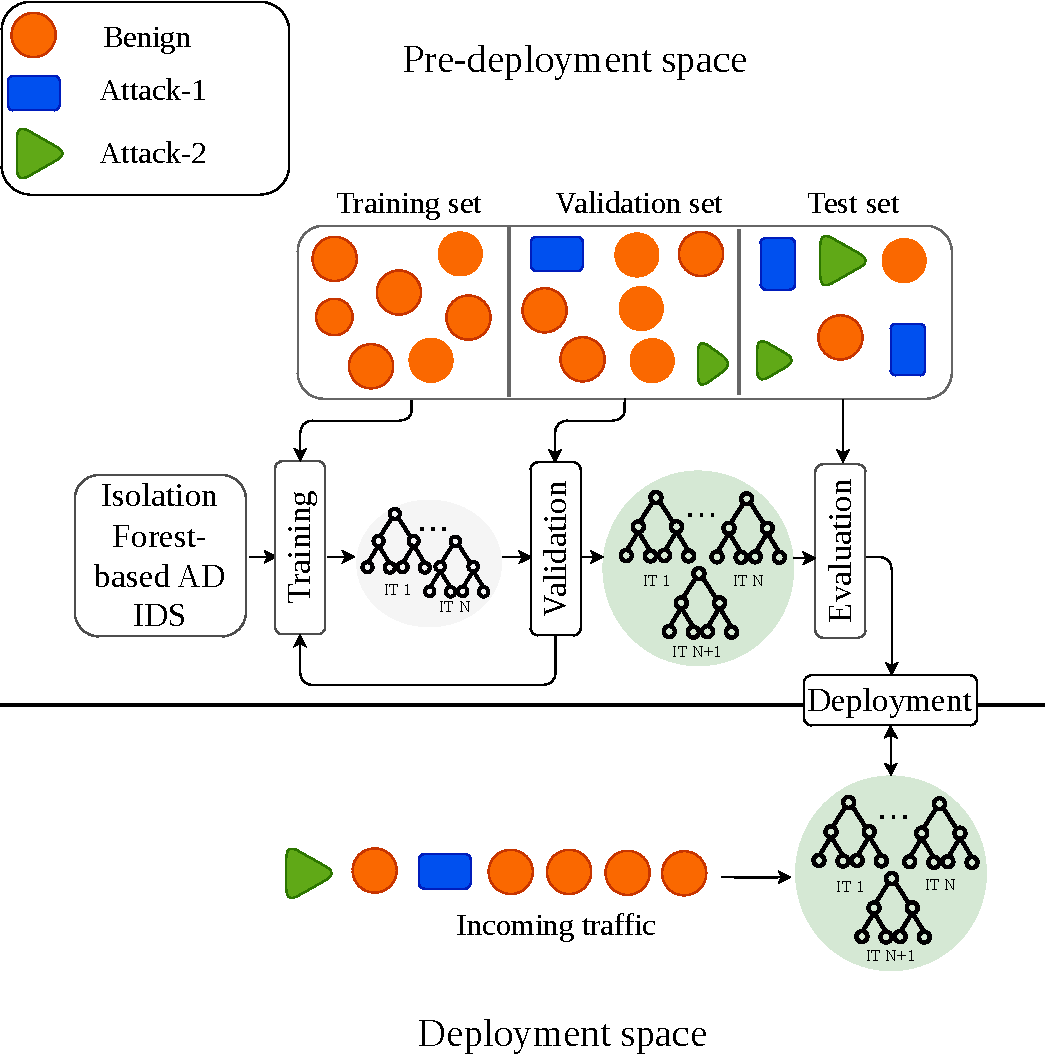
\includegraphics[width=\linewidth]{figures/introduction/ML_NIDS_4-crop}%
                    };
                    \begin{scope}[x={(img.south east)},y={(img.north west)}]
                        \draw[structure.fg!85!black,draw opacity=0.16,line width=5pt,line join=round]
                            (0.43,0.35)
                            .. controls (0.38,0.43) and (0.40,0.58) .. (0.49,0.67)
                            .. controls (0.59,0.76) and (0.76,0.69) .. (0.78,0.56)
                            .. controls (0.80,0.43) and (0.70,0.33) .. (0.58,0.32)
                            .. controls (0.51,0.31) and (0.46,0.31) .. cycle;
                        \path[fill=structure.fg!45,fill opacity=0.08]
                            (0.43,0.35)
                            .. controls (0.38,0.43) and (0.40,0.58) .. (0.49,0.67)
                            .. controls (0.59,0.76) and (0.76,0.69) .. (0.78,0.56)
                            .. controls (0.80,0.43) and (0.70,0.33) .. (0.58,0.32)
                            .. controls (0.51,0.31) and (0.46,0.31) .. cycle;
                        \draw[structure.fg!85!black,draw opacity=0.70,line width=0.9pt,line join=round]
                            (0.43,0.35)
                            .. controls (0.38,0.43) and (0.40,0.58) .. (0.49,0.67)
                            .. controls (0.59,0.76) and (0.76,0.69) .. (0.78,0.56)
                            .. controls (0.80,0.43) and (0.70,0.33) .. (0.58,0.32)
                            .. controls (0.51,0.31) and (0.46,0.31) .. cycle;
                    \end{scope}
                \end{tikzpicture}%
            }
            \label{fig:ml_nids_workflow}
        \end{figure}

    \end{columns}

    \only<5>{%
        \begin{tikzpicture}[remember picture,overlay]
            \node[anchor=south,text=structure.fg,font=\small]
                at ([yshift=0.42cm]current page.south)
                {\(\Longrightarrow\) This work focuses on the \textbf{configuration step} and its impact on \textbf{NIDS performance}.};
        \end{tikzpicture}%
    }
\end{frame}
